\documentclass[conference]{IEEEtran}
\usepackage{amsmath,amssymb,amsfonts}
\usepackage{algorithmic}
\usepackage{graphicx}
\usepackage{textcomp}
\usepackage{xcolor}
\usepackage{makecell}
\usepackage{biblatex}
\usepackage{graphicx}
\usepackage{subcaption}
\usepackage{float} % Required for [H] option
\usepackage{tikz}




\def\BibTeX{{\rm B\kern-.05em{\sc i\kern-.025em b}\kern-.08em
		T\kern-.1667em\lower.7ex\hbox{E}\kern-.125emX}}
	
\addbibresource{references.bib}


\begin{document}
	
	\title{ICS5510 Assignment}
	
	\author{\IEEEauthorblockN{Carmel Gafa}
		\date{December 2024}
		
	}
	
	\maketitle
	
	\begin{abstract}
	TODO: abstract here
	\end{abstract}
	
	\begin{IEEEkeywords}
		TODO: keywords
	\end{IEEEkeywords}
	
	\section{Introduction}

	This exercise will explore the well-known COMPAS dataset using several machine-learning techniques. We will also look into the ethical implications of predictive risk assessment models. We have taken the opportunity of this study to implement some of the techniques discussed in ICS5510, like imputation and encoding, to help in data preparation, linear regression, neural networks and others as the tools used for prediction.
	
	Wherever possible, we preferred the manual implementation of some of the steps over the functionality available in popular Python libraries to appreciate the techniques implemented more thoroughly.
	
	\subsection{History of the COMPAS tool}
	
	The COMPAS (Correctional Offender Management Profiling for Alternative Sanctions) dataset and tool have a controversial history rooted in its use for assessing the likelihood of recidivism among criminal defendants. Developed by Northpointe, COMPAS gained widespread adoption in the U.S. judicial system for pretrial risk assessments and sentencing decisions. This tool is helpful in various stages of the criminal justice process, including bail, sentencing, and parole decisions.
	
	However, in 2016, an investigative report by ProPublica revealed significant racial biases in the tool's predictions. The report found that COMPAS disproportionately labelled Black defendants as high risk for reoffending while underestimating the risk for white defendants, even when both groups had similar criminal histories. This revelation sparked a broader debate about using algorithmic tools in criminal justice and their transparency and fairness. 
	
	The COMPAS tool has not been directly the subject of lawsuits, but its use in judicial decisions has led to legal challenges. For instance, in State v. Loomis (2016), the Wisconsin Supreme Court upheld using COMPAS in sentencing. However, judges must be informed about its limitations, particularly its proprietary nature and potential biases. The case highlighted the broader tension between the utility of predictive algorithms and their application's need for accountability and fairness.
	
	\subsection{The COMPAS dataset}
	
	The dataset that originates from the COMPAS tool is widely used in criminology and machine learning studies. 
	
	The dataset contains attributes such as demographic information, prior charges, juvenile records, and risk scores, including the widely analysed decile score, which categorises individuals into ten different risk groups. 
	
	The decile score is a critical feature, assigning a numerical value to an individual's likelihood of reoffending. Other important features include the number of prior offences \textbf{\texttt{priors\_count}} and the type of offence \textbf{\texttt{c\_charge\_degree}}, provide context for these predictions. At the same time, the label \textbf{\texttt{two\_year\_recid}} indicates whether an individual reoffended within two years of their COMPAS assessment.
	
	While the dataset has been instrumental in research aimed at understanding and improving risk prediction models, it has also been the subject of extensive scrutiny due to its implications for fairness and equity in the justice system. A couple of thoughts resulting from this scrutiny include:
	
	
	\begin{itemize}
		\item Multiple studies, including the influential ProPublica investigation in 2016, have highlighted racial disparities in the COMPAS predictions. African-American defendants were found to be nearly twice as likely as Caucasian defendants to be labelled as high-risk for recidivism but not reoffend. Conversely, Caucasian defendants were more likely to be classified as low-risk but later reoffend, raising concerns about systemic bias embedded in the algorithm, which could exacerbate existing inequalities in the justice system.
	
		\item The COMPAS tool operates as a proprietary black-box model, meaning its internal workings and feature weights are not disclosed to the public or even to the defendants it evaluates. This lack of transparency prevents meaningful scrutiny and accountability, leaving users unable to fully understand or challenge the tool's predictions.
	
		\item The COMPAS algorithm relies on historical criminal justice data, which may reflect social and systemic biases. For example, law enforcement practices that can result in sentencing disparities can all influence the patterns observed in the data. Using such data as input, the COMPAS tool risks perpetuating these biases into an electronic tool.
	
		\item Some features in the COMPAS dataset, such as age and criminal history, are static and cannot change over time, as this data is based on the date of the COMPAS assessment. We can argue that these features in risk predictions without considering the period after the COMPAS assessment undermines the potential for individuals to reform and leads to insensible punitive outcomes.
	
		\item The ethical implications of using predictive algorithms in high-stakes decisions, such as sentencing and parole, constitute a significant area of concern. The potential for false positives can lead to unjustly harsher treatment, while false negatives can impact public safety.
	
		\item The dataset available for research purposes is a reduced version of the original COMPAS data, with several features anonymised or removed. Missing important data introduces limitations for academic studies aiming to replicate or validate the findings from real-world COMPAS applications.
	\end{itemize}
	
	
	The criticism of the COMPAS tool emphasises the challenges of deploying machine learning systems in sensitive domains like justice. These challenges are not unique to COMPAS but highlight broader issues in applying algorithmic decision-making tools in socially important contexts. They highlight the need for transparency, fairness-aware modelling techniques, and careful ethical evaluations when designing and implementing such tools.
	
	\subsection{Objectives of this work}
	
	The main objectives of this study are:
	
	\begin{itemize}[]
		\item Analyse the COMPAS dataset and its predictions.
		\item Prepare the dataset for machine learning through cleaning, transformation, and feature engineering.
		\item Train and evaluate machine learning models for ethical analysis.
		\item Investigate potential biases and ethical implications in predictions.
	\end{itemize}
	
	
	\section{Downloading and first look at the dataset}
	
	The COMPAS dataset used in this study is publicly available through ProPublica's GitHub repository. This repository contains the dataset and other assets used by ProPublica to investigate the biases present in the COMPAS risk assessment tool.
	
	The file chosen for this analysis is \textbf{\texttt{compas-scores-two-years.csv}}, as it provides the cleanest and most relevant data for general recidivism prediction. This CSV file contains the key data required for our study, including several attributes related to demographics, criminal history, COMPAS risk scores, and the two-year recidivism outcomes that are important for exploring the predictive capabilities and the ethical implications of machine learning models in the context of recidivism prediction. 
	
	The dataset includes important information about individuals. Following an initial analysis, a list of the key fields in the dataset is below.
	
	\begin{itemize}
	
		\item Personal Information, includes attributes such as \textbf{\texttt{age}}, \textbf{\texttt{race}}, \textbf{\texttt{age\_category}}, etc.
		
		\item Case and Event-Related Details are the fields prefixed with \textbf{\texttt{c\_}} that provide a timeline and details of a person's interactions with the criminal justice system.
	
		\item Violence Risk Assessment are the fields prefixed with \textbf{\texttt{v\_}} and are associated with the violence risk assessment in COMPAS. This dimension predicts violent recidivism risk.
	
		\item Case-Level Details for Violent Recidivism are the fields prefixed with \textbf{\texttt{vr\_}}. These fields provide additional details specific to violent recidivism events.
	
		\item Juvenile Criminal Record are the fields prefixed with \textbf{\texttt{juv\_}}. These fields capture information about an individual's juvenile criminal record, which is a key predictor of future adult criminal behaviour.
	
		\item Previous Charges and Severity can be deduced from fields such as \textbf{\texttt{priors\_count}} and \textbf{\texttt{juv\_}} fields.
	
		\item Additional fields, including \textbf{\texttt{r\_charge\_}}, \textbf{\texttt{r\_offense\_}}, \textbf{\texttt{vr\_}} fields, \textbf{\texttt{c\_charge\_degree}}, and \textbf{\texttt{c\_charge\_desc}}, provide a broader perspective on criminal history and severity.
	
	
		\item Two-Year Recidivism, or the \textbf{\texttt{two\_year\_recid}} field in the COMPAS dataset, indicates whether an individual reoffended (recidivated) within two years of their initial assessment or release. This field is critical for evaluating the predictive accuracy of the COMPAS risk assessment tool.
	
		\item Decile Score is a standardized risk score in the COMPAS dataset. It categorizes an individual's likelihood of recidivism into ten equal groups (deciles) where 1 is the lowest risk, and 10 is the highest risk. Each decile represents approximately 10\% of the sample when applied to a norm group.

	\end{itemize}

	Suppose that we observe the following data:
	
	\begin{table}[!ht]
		\centering
		\begin{tabular}{|l|l|}
			\hline
			Field & Value \\ \hline
			\textbf{\texttt{priors\_count}} & 5 \\ \hline
			\textbf{\texttt{juv\_felony\_count}} & 2 \\ \hline
			\textbf{\texttt{juv\_misdemeanor\_count}} & 3 \\ \hline
			\textbf{\texttt{r\_charge\_degree}} & Felony \\ \hline
		\end{tabular}
	\end{table}
	
	We can interpret this as an individual who has five total prior charges, including:
	
	\begin{itemize}
		\item 2 juvenile felonies
		\item 3 juvenile misdemeanours
		\item The severity of previous charges includes felonies (\textbf{\texttt{r\_charge\_degree}}).
	\end{itemize}
	

	\section{Preparing the data for further analysis and training}
	
	Before we can perform any analysis or apply machine learning techniques, it is important to pre-process and prepare the dataset so that we can handle missing values, encode categorical features, and split the data into training, testing, and validation sets. This step will produce a clean dataset for building accurate and unbiased models. The following steps outline the procedures to prepare the dataset for further analysis and training.

	
	\subsection{Initial look at data and missing values handling}
	
	The dataset has 7214 instances over 53 columns. The target of the dataset is \textbf{\texttt{decile\_score}}, but the dataset also contains information about whether or not the person recidivised, most notably through the label \textbf{\texttt{two\_year\_recid}}. 
	
	The first step in data preparation is removing the features irrelevant to this exercise or with over 50\% missing records. We removed all the COMPAS-administrative labels and additional recidivism information apart from \textbf{\texttt{two\_year\_recid}}, narrowing the dataset to 17 fields.
	
	The difference between \textbf{\texttt{c\_jail\_in}} and \textbf{\texttt{c\_jail\_out}} was calculated into a new field, \textbf{\texttt{days\_in\_jail}} and the difference between \textbf{\texttt{in\_custody}} and \textbf{\texttt{out\_custody}}, in a new field, \textbf{\texttt{days\_in\_custody}}. We subsequently removed the features containing date information from the dataset, together with \textbf{\texttt{days\_in\_custody}}, as it contained no information. At this stage, the dataset contains thirteen features: eight numerical, four categorical, and one descriptive. It also contains two labels, decile\_score, which we will treat as the leading label in this exercise and \textbf{\texttt{two\_year\_recid}}, which we are keeping to compare the prediction power of our models to the original one.
	
	
	\subsection{Imputation of missing data}
	
	While examining the resultant dataset, we noticed that \textbf{\texttt{days\_b\_screening\_arrest}} has  6907 values that are not null. Whilst it is possible to eliminate the rows that contain the null values at this stage, we replaced the missing values using a KNN imputation technique by grouping the numeric values of this dataset so that we can calculate the missing values. We checked this process by plotting the distribution of \textbf{\texttt{days\_b\_screening\_arrest}} before and after imputation to see if any variations occurred.
	
	\begin{figure}[h!]
		\centering
		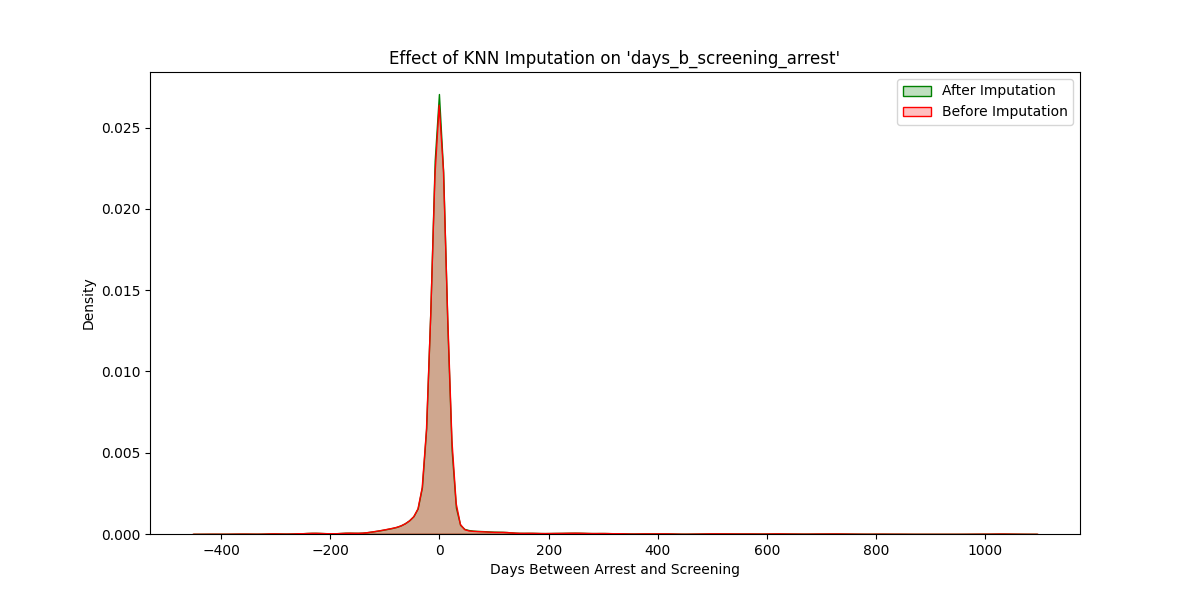
\includegraphics[width=0.9\linewidth]{img/imputation}
		\caption[Distribution \textbf{\texttt{days\_b\_screening\_arrest}} of before and after KNN imputation]{}
		\label{fig:imputation}
	\end{figure}

	At this stage, the dataset contains four categorical features that need encoding for machine learning algorithms. This section will focus on converting them into a numerical format using two encoding techniques. The categorical features and their values are listed below:
	
	\begin{table}[!ht]
		\centering
		\begin{tabular}{|l|l|l|}
			\hline
			Feature & Description & Unique Values \\ \hline\hline
			\textbf{\texttt{sex}} & Gender of the individual & \shortstack{[l]Male\\Female} \\ \hline
			\textbf{\texttt{race}} & Race of the individual & \shortstack[l]{African-American\\Caucasian\\Hispanic\\Asian\\Native American\\Other} \\ \hline
			\textbf{\texttt{age\_cat}} & Age category & \shortstack[l]{Less than 25\\25 - 45\\Greater than 45} \\ \hline
			\textbf{\texttt{c\_charge\_degree}} & Degree of the criminal charge & \shortstack[l]{F (Felony)\\M (Misdemeanor)} \\ \hline
		\end{tabular}
	\end{table}
	
	The following transformations are applied:
	
	\begin{itemize}[]
		\item One-Hot Encoding on \textbf{\texttt{sex}}, \textbf{\texttt{race}}, and \textbf{\texttt{c\_charge\_degree}}, transforming them into binary columns.
		\item Ordinal Encoding on \textbf{\texttt{age\_cat}}. This encoding technique was preferred over one-hot in this case as it preserves order,thus respecting the inherent ranking of the category.
    \end{itemize}
	 	
	The original categorical columns were retained in the dataset for future use in the analysis steps. 
	
	\subsection{Splitting the data into train, test and dev}
	
	A stratified shuffle split technique is preferred to create the train, test, and dev datasets whilst ensuring that the splits are proportional by \textbf{\texttt{race}}. In the first split, 80\% Train and 20\% Test are created, whilst in the Second split, The 20\% Test is further divided into 10\% Test and 10\% Dev.


	\section{Data exploration and visualisation}
	
	This section will examine the dataset in more detail to understand the patterns, distributions, and relationships. In this exercise, we will use more of the visual tools available through several Python libraries to identify potential biases, explore correlations between variables, and uncover insights that may influence the outcomes of predictive models. 
	
	\subsection {Demographic analysis}
	
	We begin this analysis by segmenting the dataset based by race and gender.
	
	
	% First image
	\begin{figure}
		\centering
		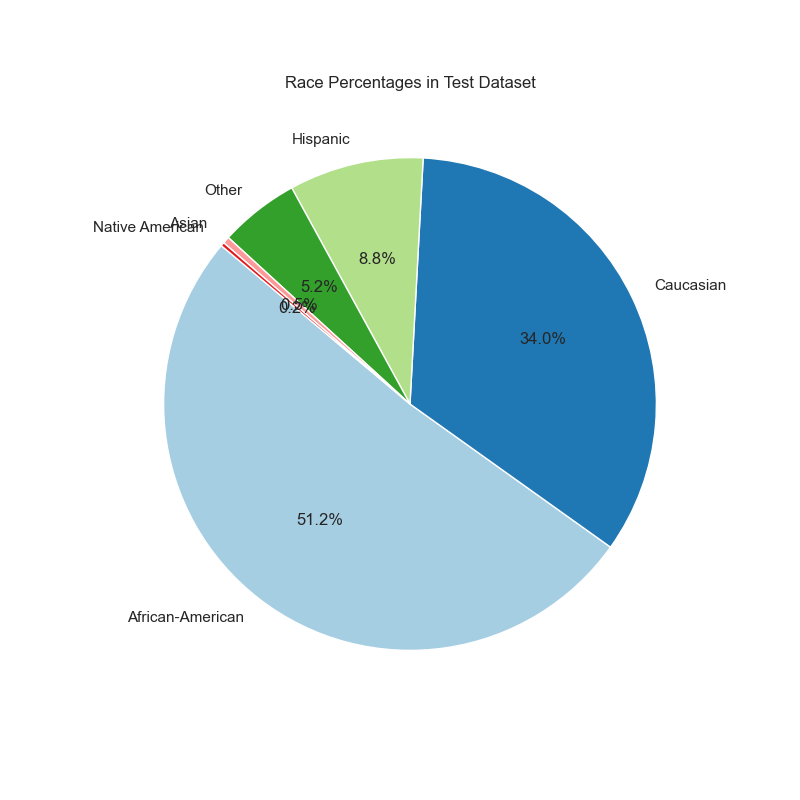
\includegraphics[width=0.7\linewidth]{img/race_percentages_pie.png}
		\caption{Caption for the first image}
		\label{fig:image1}
	\end{figure}
	\hfill
	% Second image
	\begin{figure}
		\centering
		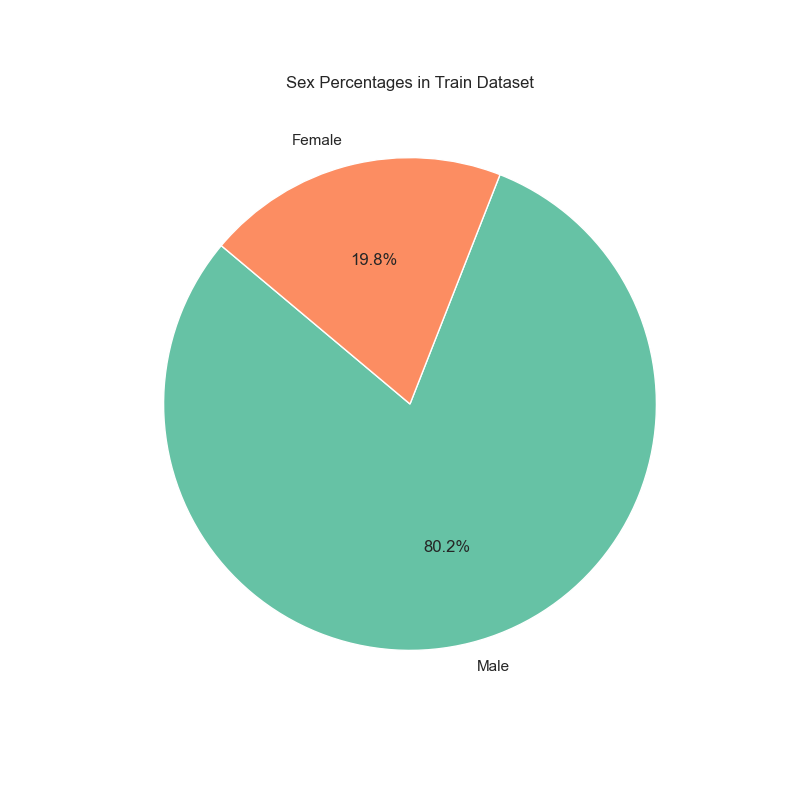
\includegraphics[width=0.7\linewidth]{img/sex_percentages_pie.png}
		\caption{Caption for the second image}
		\label{fig:image2}
	\end{figure}

	
	By examining the racial composition of the dataset, we observe the following:
	
	\begin{itemize}
		\item Over half of the test dataset is composed of African-American individuals, suggesting that the dataset may be imbalanced, with a disproportionate representation of one racial group.
		\item Asians and Native Americans each makeup only 0.2\% of the dataset; this underrepresentation might raise some concerns as it may lead to challenges in statistical analysis or machine learning models. Such concerns include the lack of reliability or significance for these groups due to insufficient data.
	\end{itemize}
		
	Figure \ref{fig:race-sex-breakdown} also shows our dataset's male/female split, with females comprising only 19.8\%. It is, therefore, evident that the female group is underrepresented, which can lead to biased models as models may overfit male patterns and underperform on females and misleading conclusions as insights derived might generalise poorly for the female subgroup.
	
	
	\subsection{Age distribution analysis}
	

	We used a boxplot to illustrate the age patterns across racial groups, helping to identify central values, spread, and any anomalies.

	\begin{figure}[H]
		\centering
		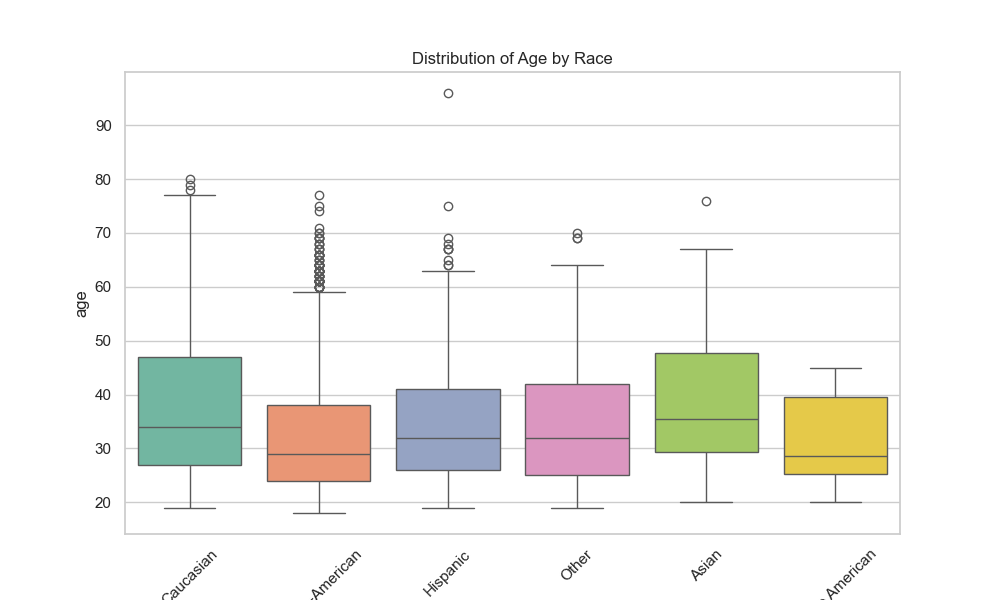
\includegraphics[width=0.9	\linewidth]{img/age_by_race_boxplot}
		\caption{}
		\label{fig:age-by-race-boxplot}
	\end{figure}
	


	\begin{table}[H]
		\centering
		\begin{tabular}{|l|l|p{4cm}|}
			\hline
			Race & Median Age & Distribution Description \\ \hline \hline
			African-American & $\approx$30 years & Concentrated in the 20–40 range, with a relatively narrow spread. We notice outliers above 60 years,  indicating fewer older individuals. \\ \hline
			Caucasian & $\approx$40 years & Broader age range, from 20 to 70+ years. We notice more older individuals (upper outliers), making this group appear older on average. \\ \hline
			Hispanic & $\approx$30–35 years & Moderately broad spread, with most individuals between 20 and 50 years. \\ \hline
			Asian & $\approx$30 years & Narrow distribution, concentrated between 25 and 40 years. No outliers. \\ \hline
			Native American & $\approx$33 years & Very tight distribution, with all ages clustered closely around the median (little variability). It is important to note that this group accounts for a tiny portion of the population. \\ \hline
			Other & $\approx$35–40 years & Similar to Caucasians but with slightly fewer older individuals. The IQR shows a widespread. \\ \hline
		\end{tabular}
	\end{table}



	\subsection{Analysing distributions}


	Next, we plotted the distributions of all the features in our dataset; this is depicted in Figure \ref{fig:distribution-plots} . From these histograms, we notice 
	\begin{itemize}
		\item The age distribution shows a right-skewed pattern, with most individuals falling in the younger age ranges (20–40 years).
		
		\item There is a significant over-representation of certain racial groups, particularly African Americans, which could indicate potential biases in the dataset's sampling.
		
		\item Most individuals have zero juvenile felony counts, zero juvenile misdemeanour counts, and no recorded "other" juvenile offences, with each distribution rapidly declining for higher counts.
		
		\item A large proportion of individuals have a low number of prior offences, but there is a long tail indicating some individuals have a significant number of priors.
		
		\item Most individuals have relatively short jail durations, with a few experiencing significantly longer durations.
		
		\item The distribution of days between screening and arrest is clustered around zero, with few extreme outliers on both ends.
		
		\item The decile scores appear relatively evenly distributed, but slight patterns suggest clustering at specific score levels (e.g., lower decile scores are slightly more frequent).
		
		\item Two-year recidivism plot shows a near-equal distribution, indicating a balanced dataset for recidivism outcomes.
	\end{itemize}

	
	\begin{figure}[H]
		\centering
		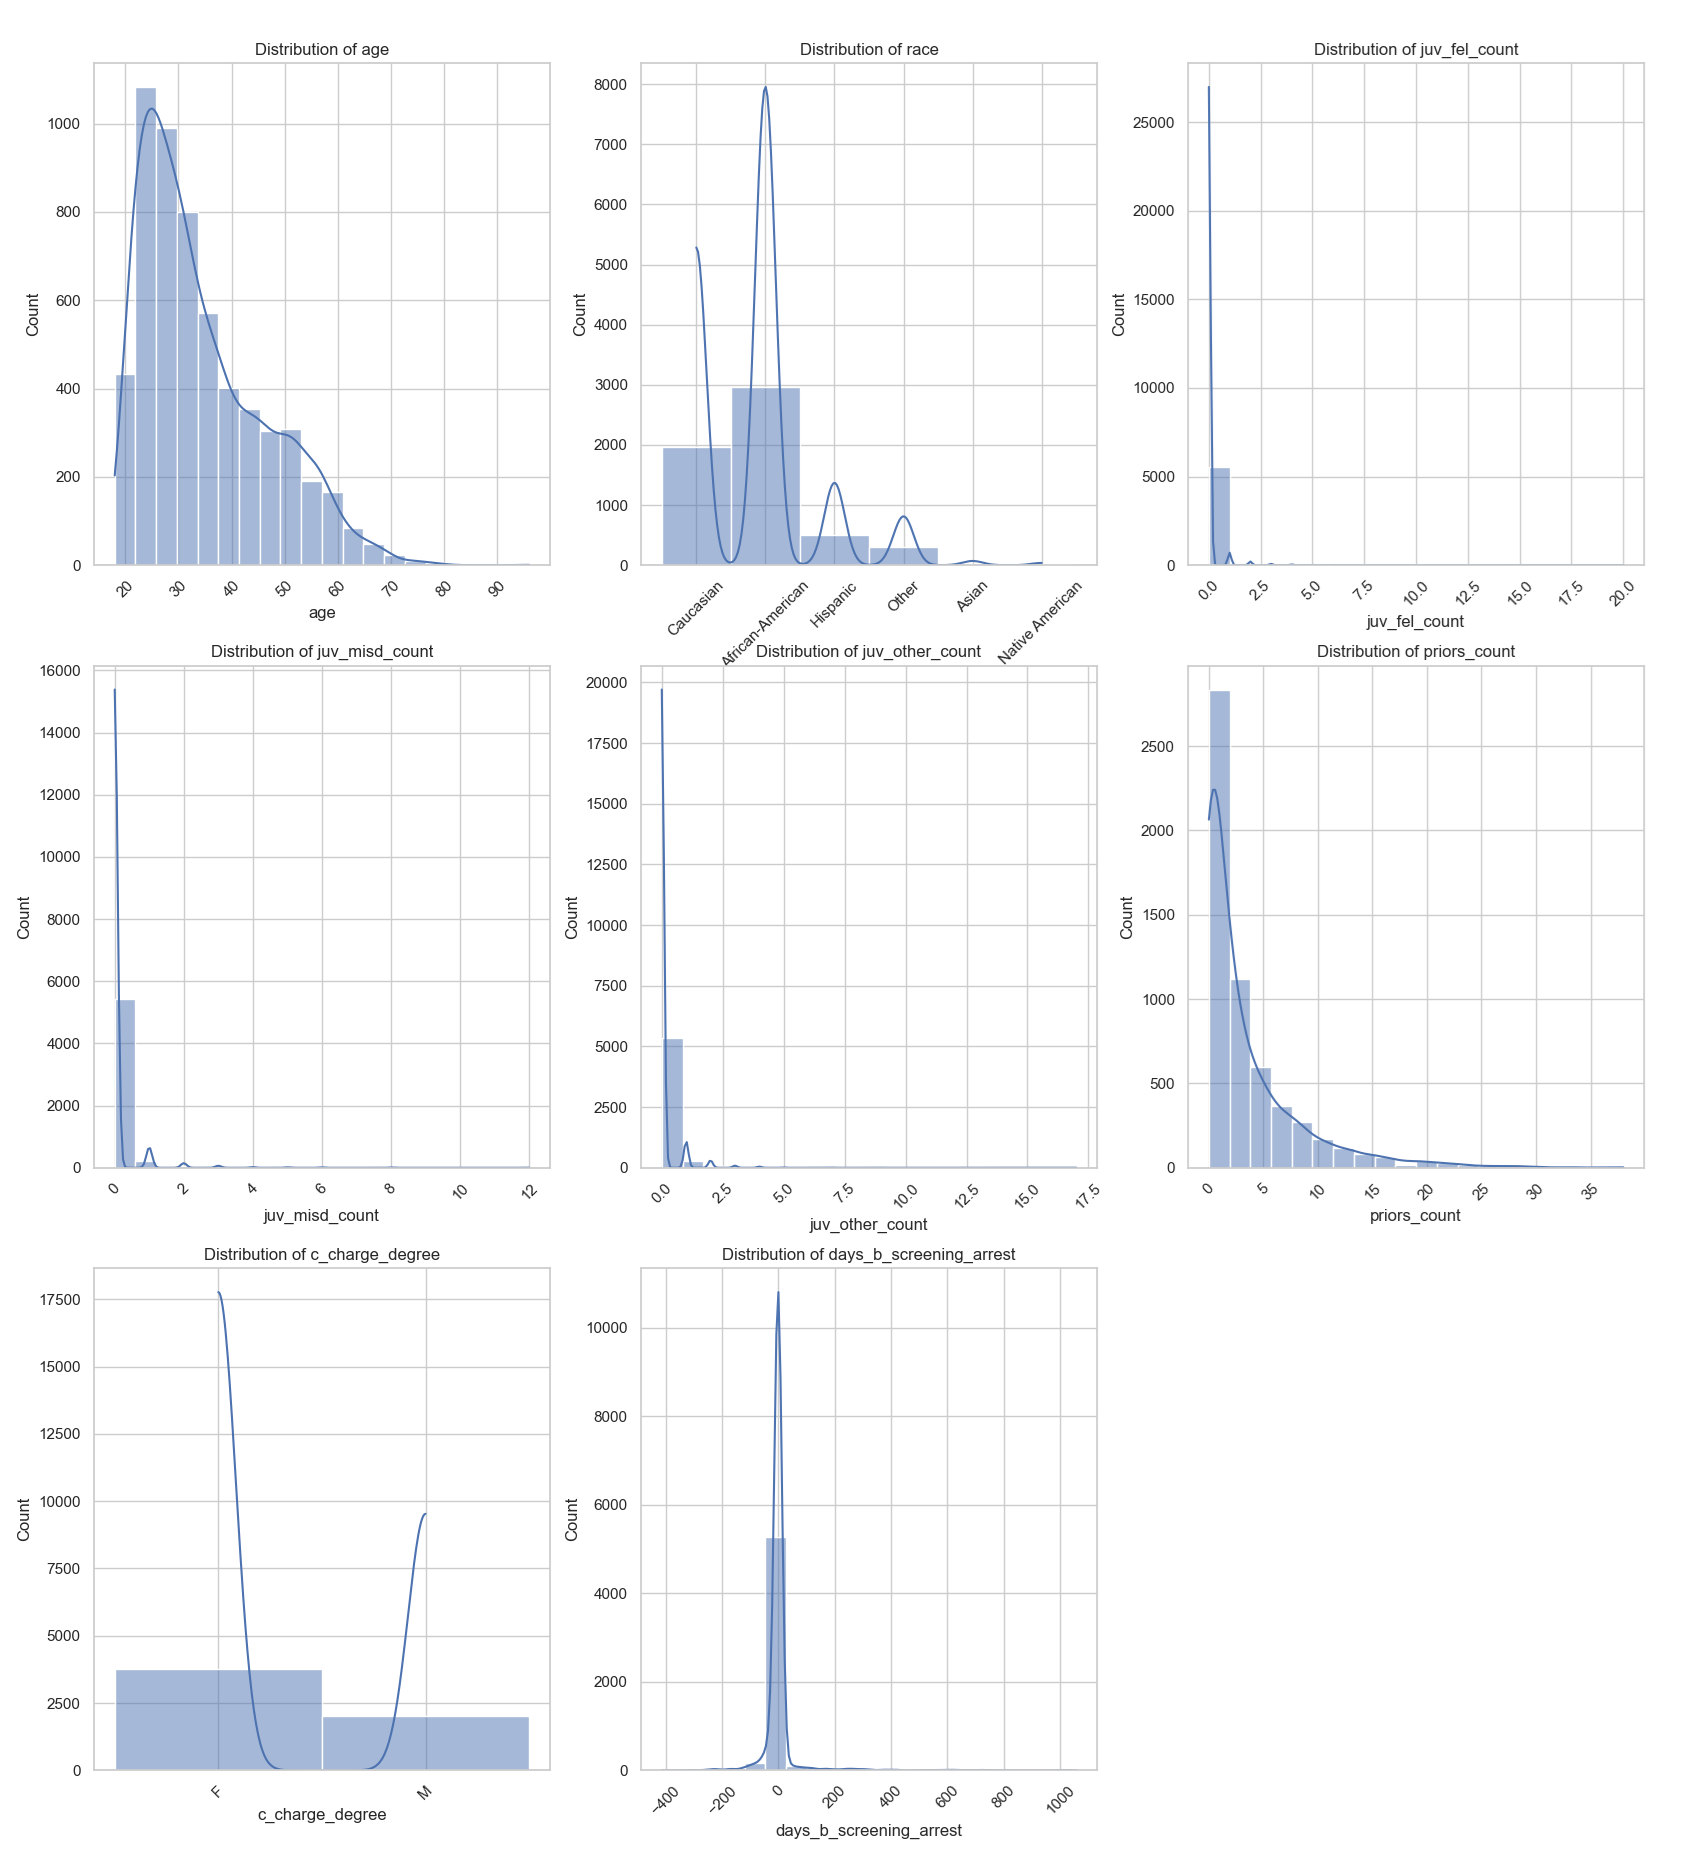
\includegraphics[width=0.9\linewidth]{img/distribution-plots}
		\caption{}
		\label{fig:distribution-plots}
	\end{figure}
	
	
	\subsection{Correlation analysis}
	
	The correlation matrix heatmap shown in Figure \ref{fig:correlationmatrixheatmap} was created to gather more insights and pinpoint the areas of high correlation. This plot raises a number of interesting observations, namely:
	
	\begin{figure}[!h]
		\centering
		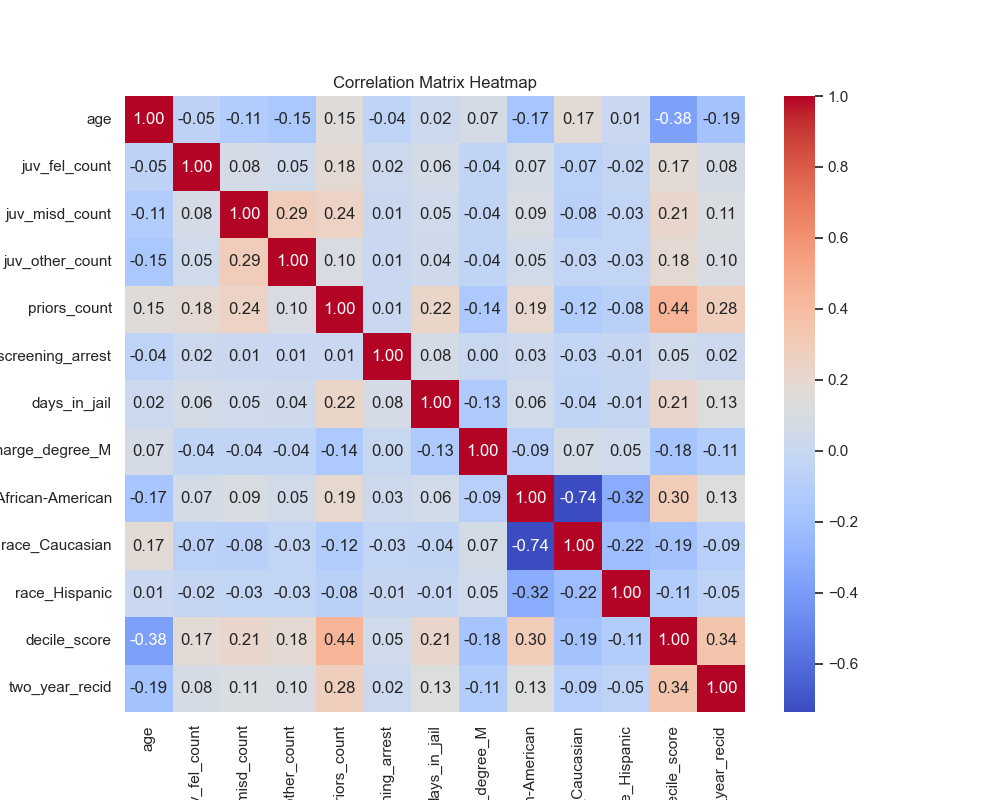
\includegraphics[width=0.7\linewidth]{img/correlation_matrix_heatmap}
		\caption{}
		\label{fig:correlationmatrixheatmap}
	\end{figure}
	
	
	\begin{itemize}
		\item Individuals with more prior offences tend to have higher risk scores, as prior criminal behaviour is a key factor in risk assessment models. The number of prior offences also correlates positively with recidivism; individuals with more prior offences tend to re-offend more often.
		
		\item Older individuals tend to have lower risk scores, suggesting that age may be inversely related to the risk of recidivism, with younger individuals being assessed as higher risk. In addition, older individuals are also less likely to recidivate, supporting this general trend.
		
		\item Individuals with higher risk scores are likelier to recidivate within two years, suggesting that the risk score (\textbf{\texttt{decile\_score}}) is predictive to a certain extent of recidivism.
		
		\item A correlation of 0.30 indicates that being African-American is moderately associated with higher decile scores, raising potential concerns about racial bias in the scoring system. At the same time, Caucasian individuals correlate -0.19 and, therefore, are less likely to receive higher risk scores.
		
		\item The time spent in jail has only a small positive relationship with the likelihood of re-offending within two years
		
		\item  Juvenile felony, misdemeanour, and other counts are positively correlated, indicating that individuals with one type of juvenile record will often have other types.
	\end{itemize}
	
	Figure \ref{fig:pairplot} is a pair plot created to substantiate these observations further to show the relationships among the selected numerical features, with the recidivism outcome (\textbf{\texttt{two\_year\_recid}}) as the hue.
	
	\begin{figure}
		\centering
		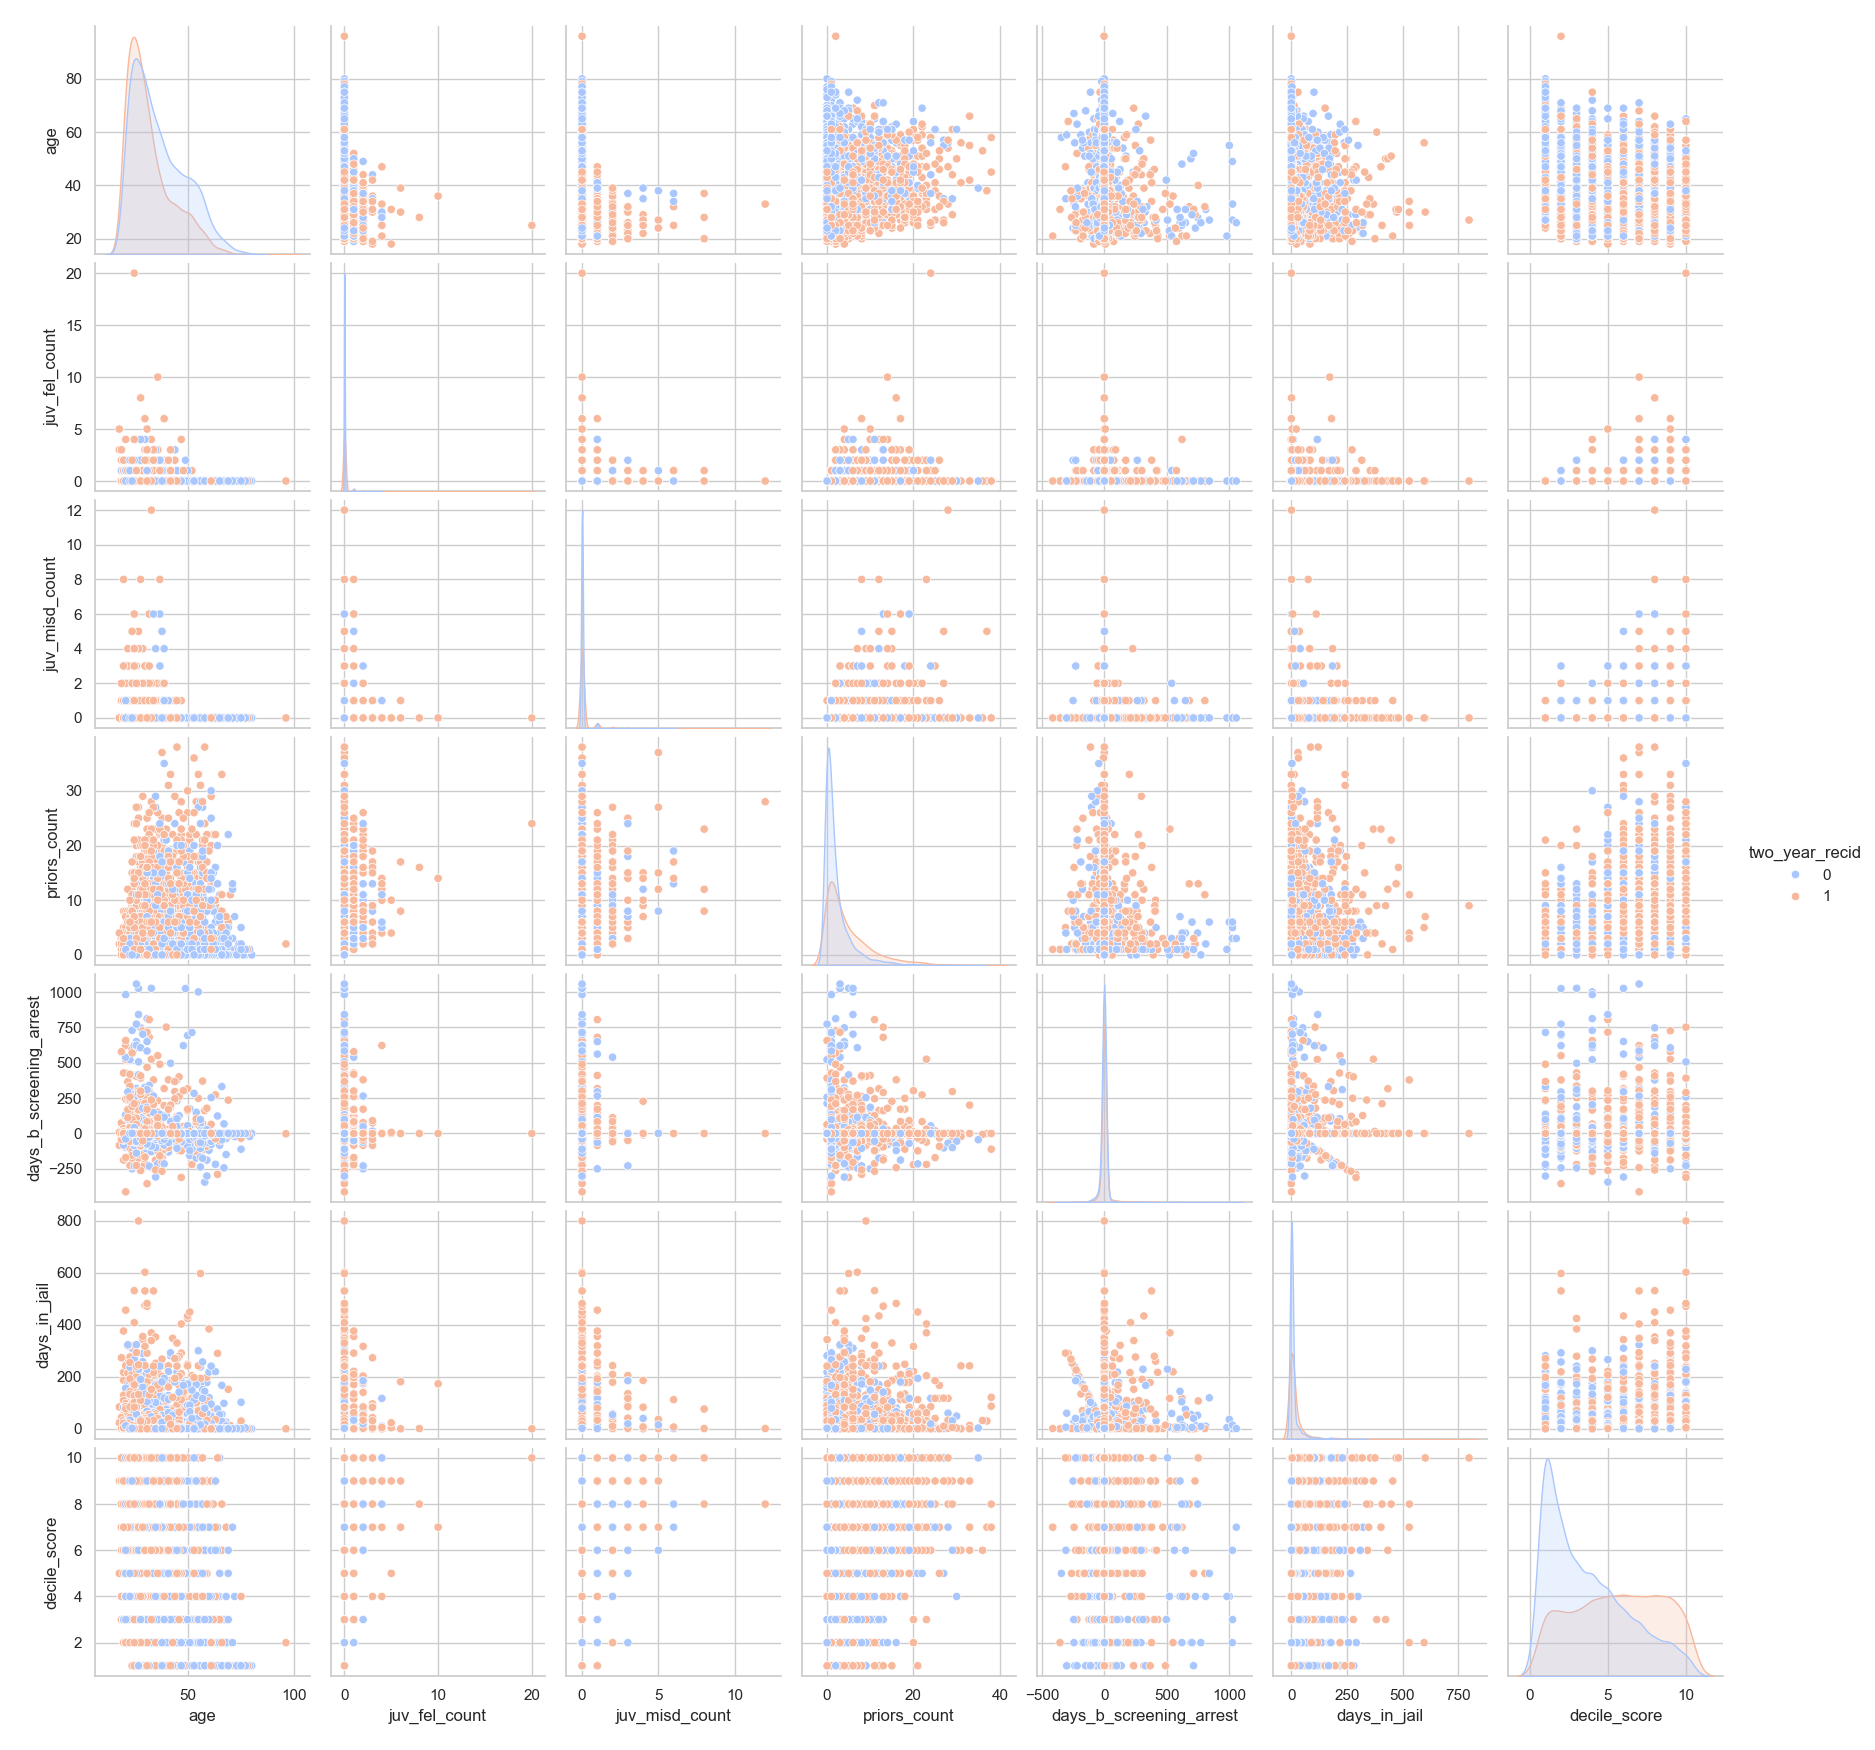
\includegraphics[width=0.7\linewidth]{img/pair_plot}
		\caption{}
		\label{fig:pairplot}
	\end{figure}
	
	
	\begin{itemize}
		\item \textbf{\texttt{age}} vs \textbf{\texttt{priors\_count}}. Younger individuals tend to have fewer prior offences, but the prior count is scattered as age increases, showing that younger offenders tend to continue having problems with the judicial system.
	
		\item \textbf{\texttt{age}} vs \textbf{\texttt{decile\_score}}. Older individuals tend to have lower decile scores. Younger individuals are associated with higher scores.
	
		\item \textbf{\texttt{priors\_count}} vs \textbf{\texttt{decile\_score}}. Positive trend: Higher priors count leads to higher decile scores, suggesting a strong correlation, indicating the tendency for offenders to be viewed as a risk community    
	
		\item The distribution of \textbf{\texttt{decile\_score}}. Two-year recidivists tend to cluster at higher decile scores (6–10 range). Non-recidivists are spread more evenly across scores.        
	\end{itemize}
	
	
	
	\subsection{Analysis of decile score relationship with race}
	
	The COMPAS dataset has been extensively discussed in recent years regarding the fairness of the scores assigned to individuals, especially considering the race component. Although the tool does not use race as one of the features in decile score prediction, there are concerns that race can be associated indirectly with other features. In this section, we will look at the data from the race point of view to see what patterns we can deduce from the dataset.
	
	As a first step, we create a boxplot to compare the distribution of \textbf{\texttt{decile\_score}} across different racial groups. 
	
	\begin{figure}
		\centering
		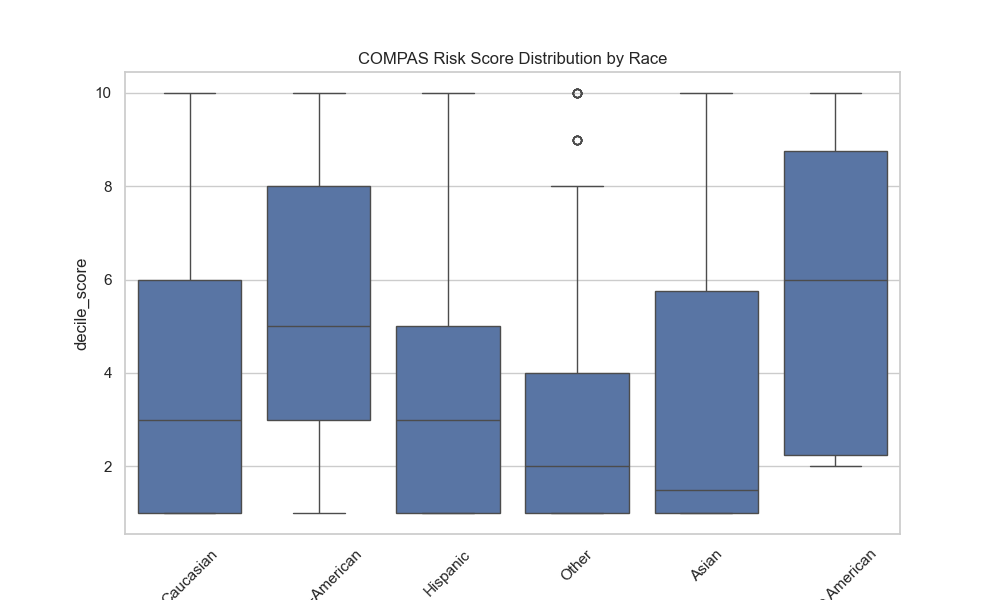
\includegraphics[width=0.7\linewidth]{img/decile_score_by_race_boxplot}
		\caption{}
		\label{fig:decilescorebyraceboxplot}
	\end{figure}
	
	
	From this plot, we notice that African Americans have higher median scores and broader distributions, which suggests a potential bias in the COMPAS scoring system. In addition, Hispanics, Asians, and Other groups scored lower on average, which may indicate differences in the risk assessment process or underlying data inputs.
	
	
	We then investigated the correlation of \textbf{\texttt{decile\_score}} with \textbf{\texttt{two\_year\_recid}} by race:
	
	\begin{figure}
		\centering
		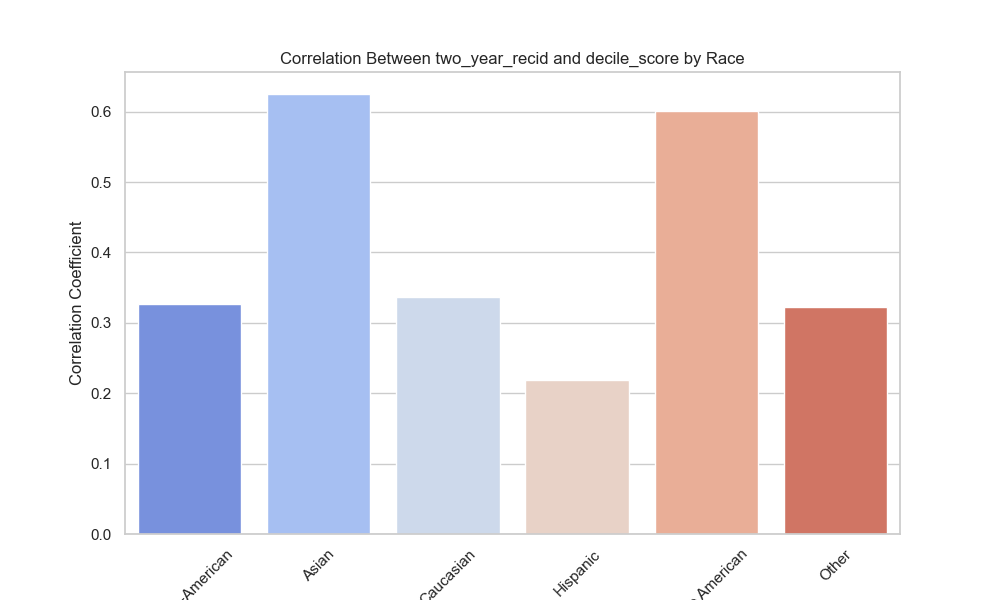
\includegraphics[width=0.9\linewidth]{img/correlation_by_race}
		\caption{}
		\label{fig:correlationbyrace}
	\end{figure}
	
	\begin{itemize}
		\item Asians and Native Americans show the highest correlations, indicating that, for these groups, COMPAS scores align more closely with observed recidivism outcomes. However, it is important to remember that these groups comprise a tiny percentage of the population.
		
		\item African-Americans, Caucasians, and Others have moderate correlations, so COMPAS scores are somewhat predictive for these groups but not as strongly as for Asians or Native Americans.
		
		\item The correlation between \textbf{\texttt{two\_year\_recid}} and \textbf{\texttt{decile\_score}} for Hispanics is 0.22, the lowest among the groups, suggesting that for Hispanic individuals, the COMPAS scores are less predictive of actual recidivism outcomes than other racial groups. The low correlation for the Hispanic group is an area of concern because if the COMPAS scores do not accurately predict recidivism for this ethnicity, this could mean that the scoring system may overestimate or underestimate their actual risk, which could lead to misclassification of individuals, leading to potential unfair treatment, for example, harsher parole conditions, sentencing).
	\end{itemize}
	
	The distribution of \textbf{\texttt{decile\_score}} for Hispanic individuals was then compared with that of other racial groups using kernel density plots (KDE). 
	
	\begin{figure}
		\centering
		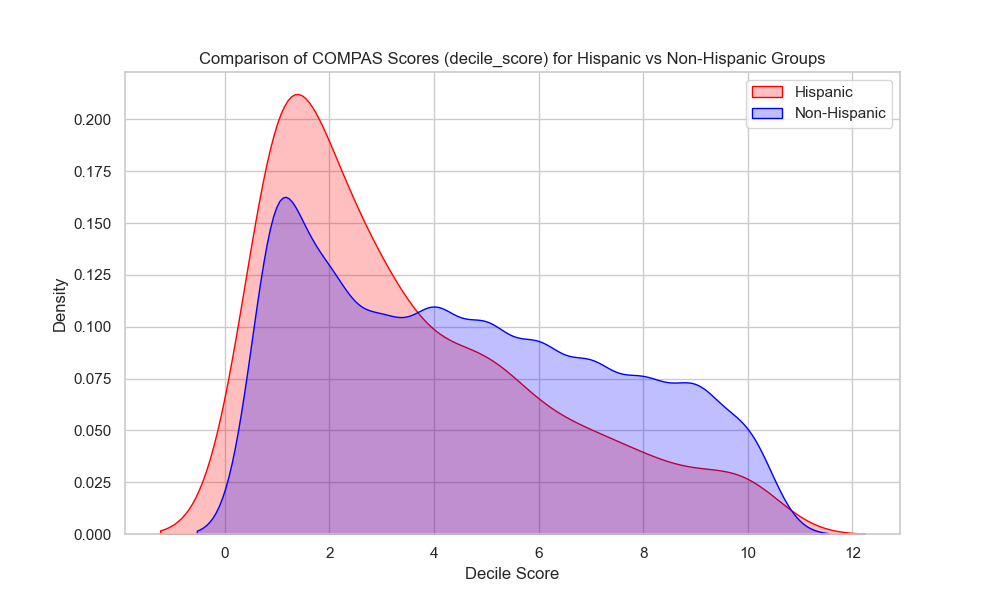
\includegraphics[width=0.7\linewidth]{img/decile_score_by_race_hispanic}
		\caption{}
		\label{fig:decilescorebyracehispanic}
	\end{figure}
	
	
	The plots show that the peak density for Hispanic individuals occurs at a lower score of around 2. In contrast, non-Hispanic individuals have a flatter distribution extending to higher scores, albeit peaking in the same region, suggesting that Hispanic individuals are more likely to receive lower COMPAS scores than non-Hispanic individuals.
	
	One has to note that we have previously seen that Hispanic individuals account for 8.8\% of the population, which is significantly smaller compared to African-American and Caucasian groups.
	Although by any means not conclusive, these aspects raise questions about how risk scores are calibrated for underrepresented groups.
	
	\subsubsection{Analysis of the African-American sector}
	
	
	We created another density plot to compare the distribution of risk scores between African-American individuals and non-African-American individuals.
	
	\begin{figure}
		\centering
		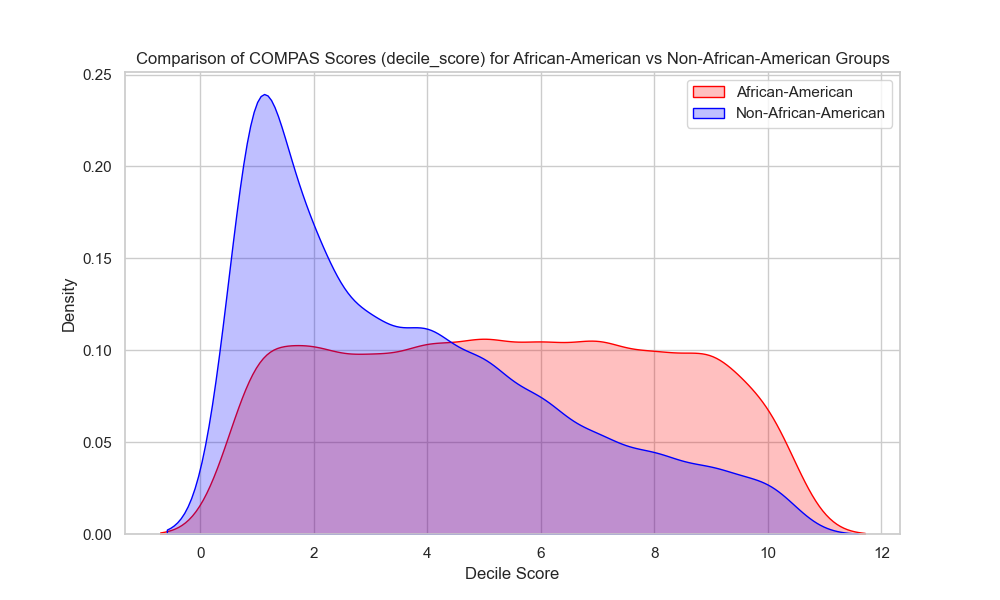
\includegraphics[width=0.7\linewidth]{img/decile_score_by_race_african_american}
		\caption{}
		\label{fig:decilescorebyraceafricanamerican}
	\end{figure}
	
	
	Here, we notice that African Americans are more likely to receive risk scores in the higher decile range, exceeding a value of six, than non-African Americans, suggesting that the COMPAS tool systematically assigns higher risk scores to African Americans. As noticed previously, non-African-American individuals show a strong peak at around a score of 2, with fewer individuals in this group receiving scores in the higher ranges.
	
	This disparity in score distributions raises concerns about potential bias in the COMPAS scoring system. African Americans appear to be disproportionately classified as higher risk, a factor which could impact downstream decisions such as sentencing or parole.
	
	\subsection{Robustness of \textbf{\texttt{decile\_score}}}
	
	As a final analysis, we compare \textbf{\texttt{decile\_score}} with \textbf{\texttt{two\_year\_recid}} to see how many high-risk individuals receded and how many individuals categorised as low-risk did not. This metric is very powerful, as it assesses the validity of the predicted risk metric. Throughout this study, we will also use this test to validate our predicted scores for the machine learning models.
	
	
	An important decision in this exercise is the selection of the decile score threshold that will dictate that values above it are more likely to recidivate and those below it not. In order to do this, we compared the decile score and two-year record for multiple thresholds. We examined the number of true negatives (the individuals with a decile score lower than the threshold and did not recidivate), true positives (those with a decile score higher or equal than the threshold and did recidivate) and false positives and negatives, and obtained the following results:
	
	\begin{table}[h!] \centering \begin{tabular}{|c|c|c|c|c|} \hline 
			\textbf{Threshold} & \textbf{True Neg} & \textbf{False Pos} & \textbf{True Pos} & \textbf{False Neg} \\ \hline 
			4                               & 2129                   & 1046                    & 964                    & 1632                    \\ \hline 5                               & 2433                   & 742                     & 1243                   & 1353                    \\ \hline 6                               & 2661                   & 514                     & 1529                   & 1067                    \\ \hline 7                               & 2849                   & 326                     & 1805                   & 791                     \\ \hline 8                               & 2979                   & 196                     & 2087                   & 509                     \\ \hline \end{tabular} \caption{Decile Score Threshold Results} \label{tab:decile_scores} \end{table}
	
	We then used these results to calculate the sensitivity, specificity, precision and accuracy:
	
	\begin{table}[h!]
		\centering
		\begin{tabular}{|c|c|c|c|c|}
			\hline
			\textbf{Threshold} & \textbf{Sensitivity} & \textbf{Specificity} & \textbf{Precision} & \textbf{Accuracy} \\ \hline
			4                               & 0.628659             & 0.670551             & 0.60941            & 0.651707          \\ \hline
			5                               & 0.521186             & 0.766299             & 0.645823           & 0.656039          \\ \hline
			6                               & 0.411017             & 0.83811              & 0.674889           & 0.645989          \\ \hline
			7                               & 0.3047               & 0.897323             & 0.708147           & 0.63074           \\ \hline
			8                               & 0.196071             & 0.938268             & 0.721986           & 0.604401          \\ \hline
		\end{tabular}
		\caption{Performance Metrics for Different Decile Score Thresholds}
		\label{tab:performance_metrics}
	\end{table}
	
	Following this procedure, a threshold of 5 was decided to provide the best balance of these metrics. With this threshold, the total accuracy and precision are moderate, indicating that while the model performs reasonably well overall, there is room for improvement. We notice a low sensitivity compared to specificity; the model is better at identifying non-recidivists than recidivists.
	
	
	The metrics for each racial group were then calculated with this threshold.
	
	
	The Caucasian group has a relatively high specificity but low sensitivity, indicating the COMPAS model more effectively avoids false positives but struggles to identify true positives. 
	
	The African-American group shows higher sensitivity but lower specificity compared to Caucasians. This suggests the model identifies more recidivists among African Americans but at the cost of more false positives.
	
	
	The Hispanic group has low sensitivity, meaning the model struggles significantly to identify true positives in this group. Precision is also the lowest, indicating a high false-positive rate.
	
	
	The significant disparity in sensitivity and specificity across racial groups highlights potential fairness issues in the model's predictions. For example, the model disproportionately favours Caucasians and Asians in terms of specificity while penalizing African-Americans with higher false-positive rates.
	
	\section{Predicting \textbf{\texttt{decile\_score}} using linear regression}
	
	
	\section{Logistic regression}
	
	
	Logistic regression is a machine learning algorithm commonly used for binary classification tasks.
	
	Given a feature vector $X \in \mathbb{R}^{n_x}$, the goal of logistic regression is to predict the probability $\hat{y}$ that a binary output variable $y$ takes the value 1, given $X$, that is $\hat{y} = P(y=1|X)$, $0\le y\le1$. 
	For example, in the case of image classification, logistic regression can be used to predict the probability that an image contains a cat.

	\begin{figure}[H]
		\centering
			\begin{tikzpicture}
		\usetikzlibrary{calc}
		% Draw the ellipse
		\draw  (-0,0) circle (2);
		% Node at the center of the ellipse
		\node[circle, inner sep=0pt] (v2) at (-0,0) {};
		% Nodes for the lines
		\node (v1) at (-5, 2) {$x_1$};
		\node (v3) at (-5,0) {$x_2$};
		\node (v4) at (-5,-2) {$x_n$};
		\node (v7) at (4,0) {$\hat{y}$};
		% Draw lines stopping at the ellipse
		\draw[-] (v1) -- ($(v2)!0.37!(v1)$);
		\draw[-] (v3) -- ($(v2)!0.4!(v3)$);
		\draw[-] (v4) -- ($(v2)!0.37!(v4)$);
		\draw[-] (v7) -- ($(v2)!0.5!(v7)$);
		\node (v5) at (0,2) {};
		\node (v6) at (0,-2) {};
		\draw  (v5) edge (v6);
		\node [font=\tiny] at (-1,0) {$z=\textbf{W}^T\textbf{X}+b$};
		\node [font=\tiny] (v8) at (1,0) {$\hat{y}=\sigma(z)$};
		\node at (-3,1.5) {$w_1$};
		\node at (-3,0.25) {$w_2$};
		\node at (-3,-1.5) {$w_n$};
		\node at (-3,-0.5) {$\vdots$};
\end{tikzpicture}

		\caption{A logistic regression model}
		\label{fig:logisticregression}
	\end{figure}

	
	Logistic regression can be visualized as the model shown in Figure \ref{fig:logisticregression}. It consists of several main components:
	
	\begin{itemize}[]
		\item Inputs. The input vector to the model $\textbf{X} \in \mathbb{R}^{n_x}$.

		\item Parameters. A weight vector $\textbf{W} \in \mathbb{R}^{n_x}$ and a bias term $b \in \mathbb{R}$.  These will form the coefficients of a linear equation that gives the log odds ratio.

		\item Pre-activation result: The result is obtained by multiplying the transpose of the weights with the inputs and then adding the bias. 
		$$z= \textbf{W}^{T}\textbf{X} + b = \begin{bmatrix} w_1 & w_2 & \dots & w_n\end{bmatrix}\begin{bmatrix} x_1\\ x_2 \\ \vdots \\x_n\end{bmatrix} + b$$
		
	
		\item Sigmoid function. A function as shown in Figure \ref{fig:sigmoid}, $\sigma(z) = \frac{1}{1 + e^{-z}}$, which maps any real number $z$ to the range $(0,1)$. This function is used to ensure that the predicted probability $\hat{y}$ is always between 0 and 1.
		\begin{figure}
			\centering
			 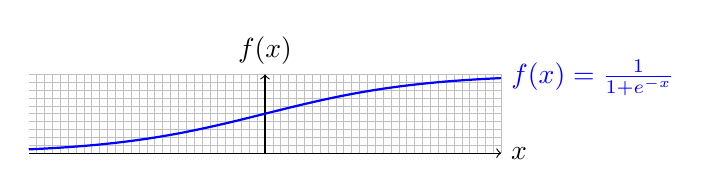
\begin{tikzpicture}[domain=-3:3] [H]% Reduced domain for a narrower plot
	% Grid and axes
	\draw[very thin,color=lightgray, step=0.1] (-3,-0) grid (3,1);
	\draw[->] (-3,0) -- (3,0) node[right] {$x$};
	\draw[->] (0,-0) -- (0,1) node[above] {$f(x)$};
	
	% Sigmoid function
	\draw[color=blue, thick, samples=100] 
	plot (\x, {1/(1 + exp(-\x))}) 
	node[right] {$f(x) = \frac{1}{1 + e^{-x}}$};
\end{tikzpicture}

			\caption{Sigmoid activation function}
			\label{fig:sigmoid}
		\end{figure}

		\item Output. The predicted probability $\hat{y}$ is computed as $\hat{y} = \sigma(z) = \sigma(\textbf{W}^{T}\textbf{X} + b)$.
	\end{itemize}
	
	
	\subsection{Logits}
		
	Logistic regression models the probability $P(y = 1 \mid X)$, of the binary dependent variable $Y$ given the predictor variables $\textbf{X} = \{x_1, x_2, \dots, x_n\}$. The goal is to find a relationship between $P(y=1)$, and the predictors $\textbf{X}$.
	
	The probability is modelled using the sigmoid function:
	$$P(y = 1 \mid X) = \frac{1}{1 + e^{-\eta}}$$
	
	Where:
	$\eta = b + w_1 x_1 + w_2 x_2 + \dots + w_n x_n$  is the linear regression function
	
	The odds of $y=1$ are defined as the ratio of the probability of success to the probability of failure:
	
	$$\text{Odds} = \frac{P(y = 1)}{1 - P(y = 1)}$$
	
	Taking the natural logarithm of the odds gives the [[log-odds-ratio]] or logit:
	
	$$\text{Log-Odds} = \ln\left(\frac{P(y = 1)}{1 - P(y = 1)}\right)$$
	
	From the sigmoid function, we can derive the relationship between the probability and the [[log-odds-ratio]]:
	
	$$P(y = 1) = \frac{1}{1 + e^{-\eta}}$$
	$$1 - P(y = 1) = 1 - \frac{1}{1 + e^{-\eta}} = \frac{e^{-\eta}}{1 + e^{-\eta}}$$
	
	The odds, therefore, are
	$$\text{Odds} = \frac{P(y = 1)}{1 - P(y = 1)} = \frac{\frac{1}{1 + e^{-\eta}}}{\frac{e^{-\eta}}{1 + e^{-\eta}}} = e^{\eta}$$
	
	
	Taking the natural logarithm of both sides gives the log-odds:
	
	$$ln\left(\frac{P(y = 1)}{1 - P(y = 1)}\right) = \eta$$
	
	Substituting $\eta = b + w_1 x_1 + w_2 x_2 + \dots + w_n x_n$
	
	\begin{equation}
		\ln\left(\frac{P(y = 1)}{1 - P(y = 1)}\right) = \eta = b + w_1 x_1 + w_2 x_2 + \dots + w_n x_n
	\end{equation}
	
	
	\subsection{Learning}
	
	The weight vector $\textbf{W}$ and the bias term $b$ are learned from a labelled training set by minimizing a suitable loss function using techniques such as gradient descent or its variants. Once trained, the logistic regression model can be used to predict the probability of the binary output variable for new input examples.
	
			
	The \textbf{feedforward process} for logistic regression can be described as follows:
	
	\begin{enumerate}[]
		\item Compute $z$ as the dot product of the weight vector $\textbf{W}$ and the input features, plus the bias term $b$, transforming the input features info a single scalar $z$ that represents the log-odds of the output being $y=1$: 
		\begin{equation}
			z= \textbf{W}^{T}\textbf{X} + b
		\end{equation}
		
		\item Pass $z$ through the [sigmoid function](neural-network-activation-functions-sigmoid.md)  to map the log-odds $z$ to a probability $\hat{y} = P(y = 1 \mid X)$, ensuring the output is between 0 and 1: 
		\begin{equation}
			\hat{y} = \sigma(z) = \frac{1}{1 + e^{-z}}
		\end{equation}

		\item During training, we define the loss function $\mathcal{L}$ as the negative log-likelihood of the predicted output given the true label: 
		\begin{equation}
			\mathcal{L} = -\left(y\ln(\hat{y}) + (1-y)\ln(1-\hat{y})\right)
		\end{equation}
	\end{enumerate}
	
	For a trained system, we compare $\hat{y}$ to a threshold to convert the probabilistic output into the final binary classification.
	
	\bigskip
	
	We now look at \textbf{feedback process} for logistic regression. To optimize the weight vector $\textbf{W}$, one standard method is to compute the derivatives of the loss function with respect to each weight and the bias term and use these derivatives to update the weights in the opposite direction of the gradient. This is known as gradient descent.
	
	To compute the derivatives, we use the chain rule of derivatives:
	
	$$
	\frac{\partial\mathcal{L}}{\partial w_i} =
	\frac{\partial\mathcal{L}}{\partial \hat{y}} \cdot
	\frac{\partial \hat{y}}{\partial z} \cdot
	\frac{\partial z}{\partial w_i}
	$$ and
	$$
	\frac{\partial\mathcal{L}}{\partial b} =
	\frac{\partial\mathcal{L}}{\partial \hat{y}} \cdot
	\frac{\partial \hat{y}}{\partial z} \cdot
	\frac{\partial z}{\partial b}
	$$
	
	We can then use these derivatives to update the weights as follows:
	
	
	\begin{equation}
		w_i \leftarrow w_i - \alpha \frac{\partial \mathcal{L}}{\partial w_i}
	\end{equation}
	
	and
	
	\begin{equation}
		b \leftarrow b - \alpha \frac{\partial \mathcal{L}}{\partial b}
	\end{equation}
	
	
	Where $\alpha$ is the learning rate, which controls the step size of the updates. By iteratively performing these updates on a training set, we can find the optimal weight vector $\textbf{W}$ that minimizes the loss function on the training set.
	
	\bigskip
	
	To calculate the derivatives, let us begin by computing the derivative of the loss function with respect to the predicted output $\hat{y}$:
	
	
	$$
	\frac{\partial \mathcal{L}}{\partial\hat{y}} = 
	\frac{\partial}{\partial\hat{y}} 
	\left(  
	-\left(y\ln(\hat{y}) + (1-y)\ln(1-\hat{y})\right)
	\right) 
	$$
	since 
	$$\frac{d \space (ln (x))}{dx}  = \frac{1}{x}$$we get:
	$$\frac{\partial \mathcal{L}}{\partial \hat{y}} = - \left( \frac{y}{\hat{y}} - \frac{1-y}{1-\hat{y}} \right) $$
	
	The derivative of the predicted output $\hat{y}$ with respect to $z$ is solved using the quotient rule that is 
	$$
	\frac{d}{dx} \left( \frac{f(x)}{g(x)} \right) = \frac{f'(x)g(x) - g'(x)f(x)}{g^2(x)}
	$$
	
	If we let
	
	\begin{table}[!ht]
		\centering
		\begin{tabular}{|l|l|l|}
			\hline
			$f(z) = 1$ & $f'(z) = 0$ \\ \hline
			$g(z)=1 +e^{-z}$ & $g'(z)= -e^{-z}$ \\ \hline
			\end{tabular}
	\end{table}

	using the derivative quotient rule,
	
	\begin{align*}
		\frac{\partial\hat{y}}{\partial z} 
		& = \frac{\partial}{\partial z} \left( \frac{1}{1 + e^{-z}} \right) \\
		& = \frac{e^{-z}}{(1 + e^{-z})^2} \\
		& = \frac{1}{(1 + e^{-z})} \space \frac{e^{-z}}{(1 + e^{-z})} \\
		& = \frac{1}{(1 + e^{-z})} \space \frac{1 + e^{-z} -1}{1 + e^{-z}} \\
		& = \frac{1}{(1 + e^{-z})} \space \left( \frac{1 + e^{-z}}{1 + e^{-z}} - \frac{1}{1 + e^{-z}} \right)\\
		& = \hat{y}(1-\hat{y})\\
	\end{align*}
	
	
	
	The derivative of $z$ with respect to $w_i$:
	
	\begin{equation}
			\begin{split}
			\frac{\partial z}{\partial w_i} 
			&=	\frac{\partial}{\partial w_i} \textbf{W}^T \textbf{X} + b\\
			&= 	\frac{\partial}{\partial w_i} (w_1 x_1 + \dots + w_ix_i+\dots+w_nx_n + b)\\
			&= x_i\\
		\end{split}
	\end{equation}
	
	Similarly,

	
\begin{equation}
	\begin{split}
		\frac{\partial z}{\partial b} 
		&= \frac{\partial}{\partial b} \textbf{W}^T \textbf{X} + b\\
		&= 	\frac{\partial}{\partial b} (w_1 x_1 + \dots + w_ix_i+\dots+w_nx_n + b)\\
		&= 1\\
	\end{split}	
\end{equation}	
	
	Therefore
	
	
	\begin{align*}
		\frac{\partial\mathcal{L}}{\partial w_i} 
		&= \frac{\partial\mathcal{L}}{\partial \hat{y}} \cdot
		\frac{\partial \hat{y}}{\partial z} \cdot
		\frac{\partial z}{\partial w_i} \\
		& = 
		-\left(
		\frac{y}{\hat{y}} - \frac{1-y}{1-\hat{y}}
		\right) \cdot
		\hat{y}(1-\hat{y})
		\cdot
		x_i\\
		&= 
		-\left(
		\frac{-y(1-\hat{y}) + (1-y)\hat{y}}{\hat{y}(1-\hat{y})}
		\right) \cdot
		\hat{y}(1-\hat{y})
		\cdot
		x_i\\
		&= \left[ (1-y)\hat{y} -y(1-\hat{y})  \right]x_i\\
		&= \left[ \hat{y} -y\hat{y} -y +y\hat{y}\right]x_i\\
	\end{align*}
	\begin{equation}
		\frac{\partial\mathcal{L}}{\partial w_i} = (\hat{y} - y) x_i
	\end{equation}
	
	and similarly
	
	\begin{equation}
		\frac{\partial\mathcal{L}}{\partial b} =
		\left(
		\hat{y} - y
		\right)
	\end{equation}
	
	
	
	
\printbibliography

\onecolumn
\pagebreak
\appendix 
\section{COMPAS dataset fields}

	\begin{table}[!ht]
	\centering
	\begin{tabular}{|l|l|l|l|l|}
		\hline
		Field Name	&	Description	&	Type	&	Options (if Categorical)	&	Used \\ \hline\hline
		\textbf{\texttt{id}}	&	Unique identifier for each individual.	&	Numeric	&	N/A	&	No \\ \hline
		\textbf{\texttt{name}}	&	Full name of the defendant	&	Text	&	N/A	&	No \\ \hline
		\textbf{\texttt{first}}	&	First name of the defendant (anonymized).	&	Text	&	N/A	&	No \\ \hline
		\textbf{\texttt{last}}	&	Last name of the defendant (anonymized).	&	Text	&	N/A	&	No \\ \hline
		\textbf{\texttt{compas\_screening\_date}}	&	Date of the COMPAS assessment.	&	Date	&	N/A	&	Yes \\ \hline
		\textbf{\texttt{sex}}	&	Gender of the defendant.	&	Categorical	&	Male, Female	&	Yes \\ \hline
		\textbf{\texttt{dob}}	&	Date of birth of the defendant.	&	Date	&	N/A	&	No \\ \hline
		\textbf{\texttt{age}}	&	Age of the defendant at the time of assessment.	&	Numeric	&	N/A	&	Yes \\ \hline
		\textbf{\texttt{age\_cat}}	&	Age category of the defendant.	&	Categorical	&	\makecell[l]{Less than 25\\25 - 45\\Greater than 45}	&	Yes \\ \hline
		\textbf{\texttt{race}}	&	Race of the defendant.	&	Categorical	&	\makecell[l]{African-American\\Caucasian\\Hispanic\\Asian\\Native American\\Other}	&	Yes \\ \hline
		\textbf{\texttt{juv\_fel\_count}}	&	Number of juvenile felony offenses.	&	Numeric	&	N/A	&	Yes \\ \hline
		\textbf{\texttt{juv\_misd\_count}}	&	Number of juvenile misdemeanor offenses.	&	Numeric	&	N/A	&	Yes \\ \hline
		\textbf{\texttt{juv\_other\_count}}	&	Number of other juvenile offenses.	&	Numeric	&	N/A	&	Yes \\ \hline
		\textbf{\texttt{priors\_count}}	&	Number of prior offenses (adult and juvenile).	&	Numeric	&	N/A	&	Yes \\ \hline
		\textbf{\texttt{days\_b\_screening\_arrest}}	&	Days between arrest and COMPAS screening.	&	Numeric	&	N/A	&	Yes \\ \hline
		\textbf{\texttt{c\_jail\_in}}	&	Jail booking date for the charge.	&	Date	&	N/A	&	No \\ \hline
		\textbf{\texttt{c\_jail\_out}}	&	Jail release date for the charge.	&	Date	&	N/A	&	No \\ \hline
		\textbf{\texttt{c\_case\_number}}	&	Case number associated with the charge.	&	Text	&	N/A	&	No \\ \hline
		\textbf{\texttt{c\_offense\_date}}	&	Date of the alleged offense.	&	Date	&	N/A	&	No \\ \hline
		\textbf{\texttt{c\_arrest\_date}}	&	Arrest date for the charge.	&	Date	&	N/A	&	No \\ \hline
		\textbf{\texttt{c\_charge\_degree}}	&	Degree of the charge.	&	Categorical	&	\makecell[l]{F (Felony)\\M (Misdemeanor)}	&	Yes \\ \hline
		\textbf{\texttt{c\_charge\_desc}}	&	Description of the charge.	&	Text	&	Free text	&	No \\ \hline
		\textbf{\texttt{is\_recid}}	&	reoffended after COMPAS screening.	&	Binary	&	0 (No), 1 (Yes)	&	No \\ \hline
		\textbf{\texttt{r\_case\_number}}	&	Case number for the re-offense.	&	Text	&	N/A	&	No \\ \hline
		\textbf{\texttt{r\_charge\_degree}}	&	Degree of the re-offense charge.	&	Categorical	&	\makecell[l]{F (Felony)\\M (Misdemeanor)}	&	No \\ \hline
		\textbf{\texttt{r\_charge\_desc}}	&	Description of the re-offense charge.	&	Text	&	Free text	&	No \\ \hline
		\textbf{\texttt{r\_jail\_in}}	&	Jail booking date for the re-offense.	&	Date	&	N/A	&	No \\ \hline
		\textbf{\texttt{r\_jail\_out}}	&	Jail release date for the re-offense.	&	Date	&	N/A	&	No \\ \hline
		\textbf{\texttt{two\_year\_recid}}	&	Label: offense within two years.	&	Binary	&	0 (No), 1 (Yes)	&	Yes \\ \hline
		\textbf{\texttt{decile\_score}}	&	COMPAS risk score (1-10).	&	Numeric	&	1–10	&	Yes \\ \hline
		\textbf{\texttt{score\_text}}	&	Risk category for general recidivism.	&	Categorical	&	Low, Medium, High	&	Yes \\ \hline
		\textbf{\texttt{v\_type\_of\_assessment}}	&	Type of COMPAS assessment conducted.	&	Text	&	Risk of Recidivism	&	No \\ \hline
		\textbf{\texttt{v\_decile\_score}}	&	Violent recidivism COMPAS score (1-10).	&	Numeric	&	1–10	&	No \\ \hline
		\textbf{\texttt{v\_score\_text}}	&	Risk category for violent recidivism.	&	Categorical	&	Low, Medium, High	&	No \\ \hline
		\textbf{\texttt{start}}	&	Start date of the two-year recidivism period.	&	Date	&	N/A	&	No \\ \hline
		\textbf{\texttt{end}}	&	End date of the two-year recidivism period.	&	Date	&	N/A	&	No \\ \hline
		\textbf{\texttt{event}}	&	offense during the two-year period.	&	Binary	&	0 (No), 1 (Yes)	&	No \\ \hline
	\end{tabular}
\end{table}






\end{document}
